\chapter{An Example Application: Deriving Behavior from Personality}\label{ch:applications}

In this chapter we present an application of language-integrated reinforcement learning to the problem of personality simulation. Creating artificial intelligent agents that are high-fidelity simulations of natural agents will require that behavioral scientists be able to write code themselves, not merely act as consultants with the ensuing knowledge acquisition bottleneck. However, translating personality models into the concrete behavior of an agent using currently available programming constructs would require a level of code complexity that would make the system inaccessible to behavioral scientists.  What we need is a way to derive the concrete actions of an agent directly from psychological personality models.  This chapter describes a reinforcement learning approach to solving this problem in which we represent trait-theoretic personality models as reinforcement learning agents.  We validate our approach by creating a virtual reconstruction of a psychology experiment using human subjects and showing that our virtual agents exhibit similar behavior patterns. Note that this work was conducted and published before we finished the Arbi-Q command arbitration algorithm of Chapter \ref{ch:arbiq}, so the AFABL agents used the Greatest-Mass q-decomposition algorithm. We have also updated the code from our original work to use AFABL syntax.


\subsection{Introduction}

There is tremendous interest in creating synthetic agents that behave as closely as possible to natural (human) agents.  Rich, interactive intelligent agents will advance the state of the art in training simulations, interactive games and narratives, and social science simulations.  However, the programming systems for creating such rich synthetic agents are too complex, or rather too steeped in computational concepts, to be used directly by the behavioral scientists who are most knowledgeable in modeling natural agents. Engaging behavioral scientists more directly in the authoring of synthetic agents would go a long way towards improving the fidelity of synthetic agents.

What we need is a programming language that a behavioral scientist can use to write agent programs using concepts familiar to behavioral scientists.  This task is complicated by the fact that the most popular and best understood personality models from behavioral science do not lend themselves to direct translation into computer programs.  Requiring a behavioral scientist to specify behaviors in the detail required in even the most cutting edge purpose-built programming language would plunge the would-be behavioral scientist agent programmer right into a morass of complex computational concepts that lie outside the expertise of most dedicated behavioral experts. To solve this problem we need a way to get from personality models to behaviors, to derive specific agent actions in an environment from a personality model without having to program the derivation in great detail.

In this chapter, we describe a way to model motivational factors from trait-oriented personality theory with reinforcement learning modules.  We describe a virtual agent simulation that reconstructs a human subject experiment from psychology, namely some of Atkinson's original work in achievement motivation and test anxiety, and show that our simulation exhibits the same general behavior patterns as the human subjects in Atkinson's experiments.  First, we briefly discuss relevant personality research and provide some background.

\subsubsection{Personality}

Personality is a branch of psychology that studies and characterizes the underlying commonalities and differences in human behavior. Within psychology, there are two broad categories of personality theories: processing theories, and dispositional, or trait theories. Social-cognitive and information-processing theories identify processes of encodings, expectancies, and goals in an attempt to characterize the mechanisms by which people process their perceptions, store conceptualizations, and how those processes drive their interactions with others \cite{dweck1988a-social-cognitive,cervone2009personality,cervone1999the-coherence}. A strength of processing theories, especially from a computational perspective, is that they provide a detailed account of the cognitive processes that give rise to personality and drive behavior.  This strength is also a drawback -- processing theories tend to be detailed and often low-level (though not as low-level as cognitive architectures, which we will discuss below), and this makes them less intuitive and less suited to describing personality in broad, easily understood terms.

Trait theories \cite{cervone2009personality}, the most well-known example of which is the Five-Factor model \cite{mccrae2008handbook}, attempt to identify stable traits (sometimes called ``trait adjectives'') that can be measured on numerical scales and remain invariant across situations in determining behavior.  A strength of the trait approach is that they are well-suited to describing individuals in broad, intuitive terms.  Two drawbacks of the approach are that there is not yet widespread agreement on a set of truly universal traits (or how many there are), and it is not clear how trait models drive behavior.  A promising line of research by Elliot and Thrash \cite{elliot2002approach-avoidance} is working towards solving these problems by integrating motivation into personality in a general way.  The work of Elliot and Thrash particularly supports the approach we present here, as they show that approach and avoidance motivation underpins all currently popular trait theories.

While debate continues about the merits and drawbacks of the different approaches to personality, the psychology community is also attempting to unify personality and motivation theory \cite{mischel2008handbook}. While the work we present here is focused on bridging the gap between the descriptive power of trait-oriented models and the behavior that arise from them, we consider this work to be complementary to work in encoding information processing theories.  In the future, rich computational agents may be built by combining approaches.

\subsubsection{Modeling Personality with Reinforcement Learning}

The essential idea behind modeling personality traits with reinforcement learning is that each motivational factor can be represented by a reinforcement learning module.  In psychology, the inherent desirability or attractiveness of a behavior or situation is referred to as {\em valence}.  For a person high in success approach motivation, behaviors or situations that provide an ``opportunity to excel'' will have high valence, while other behaviors will have lower valence.  The notion of valence translates fairly directly into the concept of reward in reinforcement learning.  Just as people with certain motivational factors will be attracted to high-valence behaviors, a reinforcement learner is attracted to high-reward behaviors.  This is the basis for modeling motivational factors with reinforcement learning modules.  By encoding the valence of certain behaviors as a reward structure, reinforcement learners can learn the behavioral patterns that are associated with particular motivational factors.  This is a powerful idea, because it allows an agent author to write agent code using motivational factors while minimizing the need to encode the complex mechanisms by which such factors lead to concrete behavior.

A critical aspect of trait theory is that traits can have interactive effects.  It is clear that a person who is high in achievement motivation will ``go for it'' when given the opportunity and that a person who is high in avoidance motivation will be more reserved.  But what happens when a person is high in both motivations?  Such interactive effects cannot be ignored in a credible treatment of personality, but it is hard to predict the behavioral patterns that will arise from given combinations of motivational factors.  One can imagine the code complexity that might result from trying to model such interactive effects with production rules or other traditional programming constructs.  As we demonstrate later, our reinforcement learning approach handles such interactive effects automatically.

It is important to note that we are not creating a new theory of personality.  We are creating a computational means of translating existing theories of personality from {\em psychology} (not computer science) into actions executed by synthetic agents.  We are also not committing to a particular theory from psychology, but rather supporting the general category of trait theories of personality which, until now, have not been directly realizable in computer agents.

In the remainder of this chapter we discuss some related work in agent modeling, present our virtual reconstruction of a human subject experiment using our reinforcement learning approach, and discuss the promising results and their implications for future work.


\subsection{Related Work}\label{sec:related-work}

There is a great deal of work in modeling all sorts of phenomena in synthetic agents.  Cognitive architectures provide computational models of many low-level cognitive processes, such as memory, perception, and conceptualization \cite{jones2005an-introduction,langley2008cognitive}.  Cognitive architectures support scientific research in cognitive psychology by providing runnable models of cognitive processes, support research in human-computer interaction with detailed user models \cite{john1998cognitive}, and can serve as the ``brains'' of agents in a variety of contexts.  The most notable and actively developed cognitive architectures are Soar \cite{laird2008extending} and ACT-R \cite{anderson2004an-integrated}.  Recently, some effort has gone into integrating reinforcement learning into Soar \cite{nason2008soar-rl}.  While RL is used to improve the reasoning system in Soar, we are using RL to support new paradigms of computer programming for agent systems.  In general, our work differs from and complements work in cognitive architectures in that we are drawing on psychological theory that is expressed at a much higher level of abstraction.  Cognitive psychology and AI have often built on each other.  Indeed, cognitive psychology is the basis of cognitive architectures in AI.  Our work is an attempt to bring in mainstream personality psychology as a basis for building intelligent agents, which we hope will complement the detailed models of cognitive architectures in creating rich synthetic agents.

There is a large and rich body of work in believable agents.  Mateas and Stern built on the work of the Oz project \cite{loyall1991hap} in creating a programming language and reactive--planning architecture for rich believable agents. They implemented their theory in the computer game Facade, a one-act interactive drama in which the player interacts with computer simulated characters that provide rich social interactivity \cite{mateas2004life-like}.  Gratch, Marsella and colleagues have a large body of work in creating rich simulations of humans for training simulations that incorporate models of appraisal theory and emotion \cite{gratch2005lessons,swartout2006toward}.  A distinctive feature of the work of both Mateas, et. al., and Gratch, et. al., is that they are dealing with the entire range of AI problems in creating believable agents that sense, act, understand and communicate in natural language, think, and exhibit human-like personalities.  Our work differs from other work in personality modeling in that we are not attempting to simulate personality, but using definitions of personality to drive the behavior of synthetic agents.  We want to derive behavior that is consistent with a given personality model, but not necessarily to ensure that the agent gives the appearance of having that personality.


\subsection{Experiments}

To test our claim that personality can be modeled by reinforcement learning modules, we created a population of simple two-module multiple-goal reinforcement learning agents and ran them in a world that replicated experiments carried out with humans by psychologist John Atkinson.  First we describe Atkinson's original research, and then discuss our virtual reconstruction of his experiments.

\subsubsection{Atkinson's Ring Toss Experiment}\label{sec:ring-toss}

John Atkinson was among the first researchers to study the existence and role of approach and avoidance motivation in human behavior. Prior to Atkinson's work, it was believed that test anxiety was equivalent to low achievement motivation.  However, Atkinson showed that test anxiety is actually a separate avoidance motivation, a ``fear of failure'' dimension that works against and interacts with achievement motivation \cite{atkinson1960achievement}.  To test his hypothesis, he administered standard tests of achievement motivation and test anxiety to a group of undergraduate psychology students and devised a series of experiments which examined the effort put forth in achieving success in tasks such as taking a final exam.  It is important to note that he did not measure the outcomes of the task, but rather the effort put forth in doing well in them.  Thus, his experiments examined the relationship between motivation and {\em behavior}, not necessarily competence.  One of his experiments, a ring toss game, produced results that clearly show the interplay of approach and avoidance motivation and is particularly well-suited to computer simulation.

In Atkinson's ring toss experiment, subjects played a ring toss game in which players attempted to toss a ring from a specified distance onto a peg.  Subjects made 10 tosses from any distance they wished, from 1 through 15 feet, and the distance at which each subject made each toss was recorded.  For analysis, subjects were divided into four groups according to their measures of achievement motivation and test anxiety so that the relationship between these motivations and their behavior could be analyzed.  For each of the two measures -- achievement motivation and test anxiety -- subjects were classified as either high or low, with the dividing line between high and low set at the median scores in each measure.  (For example, a H-L subject is high in achievement motivation and low in test anxiety).  Subjects were divided into four groups -- H-L, H-H, L-L, and L-H -- and the percentage of shots taken at each distance by each group was recorded. We discuss his results and our simulation below.

\subsubsection{Computational Models of Atkinson's Subjects}

We reconstructed Atkinson's ring toss experiment in a computer simulation.  We created 49 virtual agents that corresponded to each of the 49 human subjects in Atkinson's experiments, with the same distribution of high and low measures of achievement motivation and test anxiety.  Simplified code for a representative student subject is presented in Figure \ref{fig:student}.  Since we did not have access to Atkinson's source data, we modeled high motivation measures as having a mean of 1.5 and low motivation with a mean of 0.5, both with standard Normal distributions (mean = 0, variance = 1) scaled by $\frac{1}{2}$, so virtual test subjects did not all have the same measures.

\begin{figure}[h]

\begin{lstlisting}
val motivatedStudent = GmAgent(
  world = RingTossWorld,

  // Sequence of pairs where the second element of each pair
  // is the weight of the pair, corresponding to the personality
  // trait measure
  modules = Seq((achievementMotivation, 1.5 + X ~ N(0, 1) / 2),
                (testAnxiety, .5 + X ~ N(0, 1) / 2))
}
\end{lstlisting}

\caption{An agent representing a success-oriented student in Atkinson's ring toss experiment, containing two RL modules representing high achievement motivation and low test anxiety.  The code snippets presented here are simplified versions of the Scala code we used to run our experiments.}
\label{fig:student}
\end{figure}

As discussed earlier, each of the motivational dimensions of the virtual subjects was implemented with reinforcement learning modules that learned to satisfy the preference for perceived valence of behaviors (modeled as reward).  For example, in the achievement motivation module (see Figure \ref{fig:achievement}), the greater the distance from the peg, the greater the reward because it represents greater achievement.  Similarly, in the test anxiety module (see Figure \ref{fig:testanxiety}), greater reward is given to closer distances, because they minimize, or ``avoid'' the chance of failure from a long-distance toss.

\begin{figure}[h]
\begin{lstlisting}
val achievementMotivation = AfablModule(

  world = RingTossWorld,

  moduleReward = (state: RingTossState) => state match {
    case OneFootLine => 1,
    case TwoFootLine => 2,
    ...
    case FifteenFootLine => 15
  }

)
\end{lstlisting}
\caption{A reinforcement learning module representing achievement motivation.}
\label{fig:achievement}
\end{figure}

\begin{figure}[h]

\begin{lstlisting}
val testAnxiety = AfablModule(

  world = RingTossWorld,

  moduleReward = (state: RingTossState) => state match {
    case OneFootLine => 15,
    case TwoFootLine => 14,
    ...
    case FifteenFootLine => 1
  }

)
\end{lstlisting}

\caption{A reinforcement learning module representing Test Anxiety (`avoidance motive, a.k.a. ``fear of failure'').  Note that the rewards are inverted from the achievement motivation module, that is, the valence of avoiding achievement is higher.}
\label{fig:testanxiety}
\end{figure}

Internally, each personality module is implemented with the standard Q-learning algorithm \cite{sutton1998reinforcement}.  The ring toss world consists of 16 states -- a start state and one state for each of the 15 distances, and 15 actions available in each state that represent playing (making a toss) from a particular distance.  Each reinforcement learning module used a step-size parameter of $\alpha = 0.1$, a discount factor of $\gamma = 0.9$ (though discounting wasn't important given that the 15 states representing playing lines were terminal states, since each play was a training episode), and employed an $\epsilon$-greedy action selection strategy with $\epsilon = 0.2$.  (Readers familiar with reinforcement learning will also notice that this game is equivalent to a 15-armed bandit problem.)  We emphasize that the details of the reinforcement learning algorithms are not essential to modeling motivational factors, and those details are hidden inside the implementation of the modules.  Indeed a major goal of our work is to simplify the task of writing synthetic agents by taking care of such details automatically.

Recall that reinforcement learning algorithms learn an action value for each action available in a given state.  An action value for a state represents the expected total reward that can be achieved from a state by executing that action and transitioning to a successor state. For each of the modules -- Achievement and TestAnxiety -- the action values represent the learned utility of the actions in serving the motivational tendencies the modules represent.  The Student agents take into account the preferences of the modules -- represented by action values -- by summing their action values weighted by their module weights to get a composite action value for each action in a given state.  If we denote each module's action value by $Q(s, a)$ and the weights by $W$, then the composite, or overall, action value is:

\begin{align}
Q_{student}(s,a) =  & W_{Achievement} Q_{Achievement}(s,a) +\\
                   & W_{TestAnxiety} Q_{TestAnxiety}(s,a)
\end{align}

For the virtual experiments, each module -- Achievement and TestAnxiety -- was run to convergence and then the student agents simulated 10 plays of the ring toss game, just as in Atkinson's experiment.  We discuss the results of the experiment below.

\subsection{Model Validation}

A model is a set of explicit assumptions about how some system of interest works \cite{law2007simulation}.  In psychology the system of interest is (usually) a human or group of humans.  Our virtual reconstruction of Atkinson's experiments constitutes a computational representation of Atkinson's two-factor model of personality.  Thus, our agents are simulation models of Atkinson's subjects (the students in his ring toss experiment).  While the work presented here is only a proof of concept, we do hope to achieve a high level of validity as we refine our approach, so it will be useful to validate our models using techniques from simulation science \cite{law2007simulation}.

As we described earlier, Atkinson divided his subjects into four groups according to their measures (high or low) on achievement motivation and test anxiety.  For each of these four groups -- H-L, H-H, L-L, L-H -- he recorded the percentage of shots that each group took from each of the 15 distances.  We ran 10 replications of our simulation and recorded the mean percentages for each group and distance.  For each percentage mean we calculated a 95\% confidence interval.  We consider a model to be valid if the confidence intervals calculated on the simulation percentage means contain the percentages obtained by Atkinson in his experiments with human subjects.

\begin{table*}[ht]
\begin{center}

\begin{tabular}{|l||c|c|c|c|} \hline
Achievement: & High & High & Low & Low \\
Test Anxiety: & Low & High & Low & High \\  \hline
 & Atkinson & Atkinson & Atkinson & Atkinson \\
 & Simulation & Simulation & Simulation & Simulation \\
Range & Conf. Int. & Conf. Int. & Conf. Int. & Conf. Int. \\ \hline\hline
  1-7 & \bf{11}           & 26              & 18           & 32 \\
      & \bf{7.7}          & 14.0            &  5.6         &  8.5 \\
      & \bf{(4.0, 11.4)}  & (5.6, 22.4)     & ( 1.4,  9.7) & ( 4.4, 12.5)\\ \hline
8-12  & \bf{82}           & 60               & 58           & 48 \\
      & \bf{75.4}         & 69.0             & 74.4         & 80.0 \\
      & \bf{(65.1, 85.7)} & (61.1, 76.9)     & (62.0, 86.9) & (74.1, 85.9)\\ \hline
13-15 & 7                 & \bf{14}           & \bf{24}           & 20 \\
      & 16.9              & \bf{17.0}         & \bf{20.0}         & 11.5 \\
      & ( 8.8, 25.0)      & \bf{(9.4, 24.6)}  & \bf{(8.3, 31.7)} & ( 6.9, 16.2)\\ \hline
\end{tabular}
\caption{Validation Results.  For each subject group the percentage of shots taken by Atkinson's human subjects and by our simulation from each of three ranges is presented along with a 95\% confidence interval for the mean percentage of shots in 10 simulated replications of Atkinson's experiment.}
\label{tab:results}

\end{center}
\end{table*}

The validation results are presented in Table \ref{tab:results}. Atkinson analyzed his experimental data by aggregating the shots taken by subjects into three ``buckets'' representing low, medium, and high difficulty.  In Atkinson's analyses the dividing lines between the three buckets were set in four different ways with each yielding similar results.  For brevity we present the division obtained by using both geographical distance and distribution of shots about the median shot of 9.8 ft, in other words, the dividing line one would choose by inspecting the histogram for distinct regions.  This strategy resulted in the three buckets listed in the left column of Table \ref{tab:results}.  Each cell of the four subject groups -- H-L, H-H, L-L, L-H - contains the percentage of shots taken by Atkinson's subjects, the mean percentage obtained by running 10 replications of our simulation of Atkinson's experiment, and a 95\% confidence interval for the mean percentage.  While our model did not achieve formal validation, the general patterns of behavior are quite similar to Atkinson's human subject experiment, as shown in Figure \ref{fig:ring-toss-plots}, and we consider these results to be a good proof of concept.  We discuss some reasons behind these results and strategies for improvement below.

%% 8< 8< 8< 8< 8< 8< 8< 8< 8< 8< 8< 8< 8< 8< 8< 8< 8< 8< 8< 8< 8< 8< 8<

\begin{figure}[!h]
  \begin{center}
    \scalebox{.8}{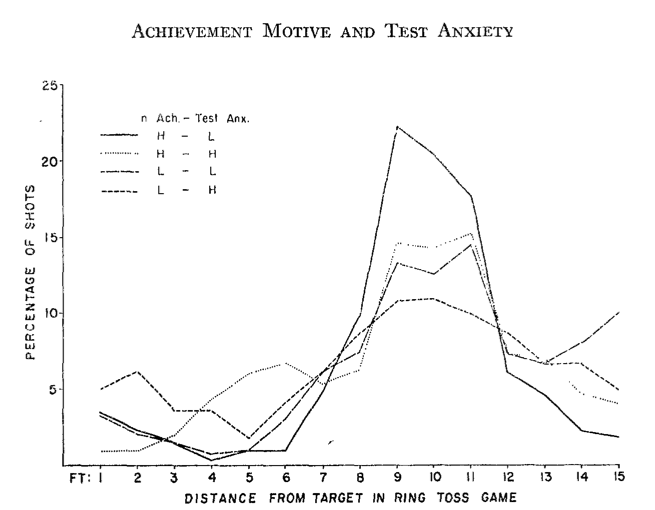
\includegraphics{atkinson}}
    \scalebox{.4}{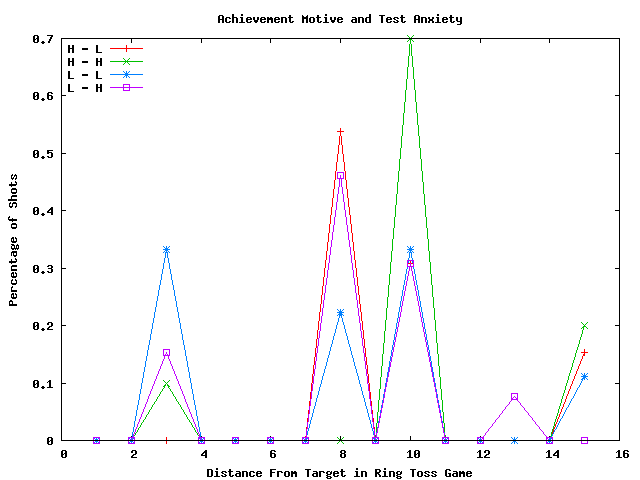
\includegraphics{iccm}}
    \caption{The top plot shows the behavior patterns of human
      subjects in Atkinson's Ring Toss experiment.  The bottom plot
      shows the behavior patterns of our synthetic agents that
      re-created Atkinson's experiment.  Note that Atkinson's plot is
      smoothed, while ours is not.}
  \end{center}
  \label{fig:ring-toss-plots}
\end{figure}

%% 8< 8< 8< 8< 8< 8< 8< 8< 8< 8< 8< 8< 8< 8< 8< 8< 8< 8< 8< 8< 8< 8< 8<

\subsection{Discussion}

We made several assumptions in our models that affected the validation results.  First, because we did not have access to Atkinson's original data, only summary presentations, we did not know the exact distribution of motivational factors among his subjects, or even the scales used in his measures.  We assumed normally distributed measures and tried several different scales before settling on the values used in the simulations reported here.  Second, it is not clear how the valence of behaviors should be translated into reward structures for RL agents.  We chose a simple linear reward structure in hopes that the system would be robust to naive encodings.  To make our approach widely useful we will need to address the manner in which reward structures are determined.

%% Third, we calculated aggregate action values by a simple weighted sum of module action values.  We are currently investigating optimal arbitration of multiple RL modules and hope to report results within the next six months.

We chose the Atkinson ring toss experiment on the advice of psychologists who recommended it as a well-known example of trait-oriented behavior theory, and because of its simplicity. However, our goal is to create large agent systems, so future work will need to address scalability -- to greater numbers of trait factors and more complex worlds -- and generalizability, or transferability, to other domains.

%% More generally, there are broader issues to be understood about
%% employing this method in practice.  From the psychology perspective, we
%% need to understand how motivational factor scales translate into the
%% weights on reinforcement learning modules, e.g., they must be
%% normalized somehow.  This issue is similar to the issue of reward
%% comparability in reinforcement learning (discussed below).  Also, our
%% example used two motivational factors.  How do we scale this approach
%% to multiple factors?  Many trait theories contain fewer traits that
%% subsume traits in other, more detailed trait theories.  We would
%% expect such decompositions to be helpful in our formulation as well.

%% The reinforcement learning algorithm employed in these experiments
%% were standard Q-learners.  While these algorithms worked well on this
%% limited problem, they likely will not be appropriate for every
%% problem.  Indeed the No Free Lunch Theorem \cite{ho2001simple} informs
%% us that each task must be matched to an appropriate algorithm -- there
%% is no universal solution to every problem.  How do we characterize the
%% matching of reinforcement learning algorithms to particular agent
%% designs and virtual worlds?

%% The algorithms we used also employed no optimization.  Reinforcement learning suffers from the curse of dimensionality, and many techniques are being actively pursued to cope with the size of state spaces for realistic-size domains.  Profitably employing reinforcement learning in agent programming systems will mean integrating scaling techniques such as function approximation (e.g., of action-value functions or state spaces) and decomposition techniques.

Finally, notice that the example code presented in this paper contains no logic for implementing behavior.  The agents and the modules are defined declaratively by specifying a state space, an action set, and a reward structure.  The run-time system derives the concrete behavior of the agents automatically from these specifications.  This technique, sometimes called partial programming or adaptive programming\cite{simpkins2008towards}, is a key concept that increases the usability of agent programming by allowing programmers to specify {\em what} an agent is to do without getting mired in {\em how} the agent should do it.

\subsection{Conclusions and Future Work}

Much work remains to make accessible personality-based agent programming systems a reality, and our work is progressing on three paths.  First, the integration of reinforcement learning into agent programming systems needs to be studied further so that we know when it is useful and how much detail can be hidden from the agent programmer. This dissertation has confirmed what we already know, namely, that authoring reward functions is not straightforward. We need to be able to specify modules in simpler terms and let the reward structure be derived automatically (we will discuss this further in Chapter \ref{ch:conclusion}. Second, the examples presented here were written together so that the reward signals of each agent were directly comparable, which allowed us to use the Greatest-Mass q-decomposition algorithm for combining the modules. Now that we have an arbitration algorithm that is robust to incomparable reward scales, we can either use a {\tt GmAgent} for personality modeling, as we have done here, or extend AFABL with weighting to enable trait-oriented personality modeling. Finally, while AFABL is currently able to handle the personality modeling presented in this chapter, AFABL is still a shallowly-embedded Scala DSL and therefore beyond the programming capabilities of most psychologists. We will need to make AFABL simpler to use. Nevertheless, reinforcement learning provides a promising approach to modeling personality traits and motivational factors in synthetic agents.  In particular, it provides us with a means to create agent programming systems that are at least comprehensible by behavioral scientists and harness their knowledge directly while minimizing the need for complex programming.
